\chapter{CÁC NGHIÊN CỨU LIÊN QUAN}\label{chapter:related_works}
\section{Mô hình mạng U-Net}
Mô hình mạng U-Net được giới thiệu trong bài báo ``U-Net: Convolutional Networks for Biomedical Image Segmentation'' vào ngày 18 tháng 5 năm 2015 bởi Olaf và các cộng sự \cite{Unet}. Tên mạng Unet xuất phát từ hình dáng chữ U của kiến trúc mạng, gồm 2 phần chính là mã hóa (Encoder) và giải mã (Decoder). Điểm đặc biệt của mạng U-Net là trong quá trình giải mã, mạng sử dụng lối tắt để kết hợp các đặc trưng được trích xuất từ các tầng tương ứng trong quá trình phần mã hóa. Bên cạnh đó, tác giả còn đề xuất hàm đánh giá mất mát có trọng số dựa trên hàm Binary Cross Entropy với mục tiêu tăng trọng số giữa các điểm biên của các tế bào. Qua đó kết quả phân đoạn tế bào được làm tốt hơn đáng kể.

\subsection{Kiến trúc mạng}
Kiến trúc mạng bao gồm 2 phần chính: phần mã hóa và phần giải mã. Phần mã hóa dựa theo kiến trúc cơ bản của mạng tích chập nơ-ron. Sáu thao tác chính trong mạng Unet bao gồm: Phép tích chập, phép pooling, phép concatetation (kết hợp), phép crop, phép up-conv (deconvolution) và phép ReLU.

\begin{figure}[H]
    \centering
    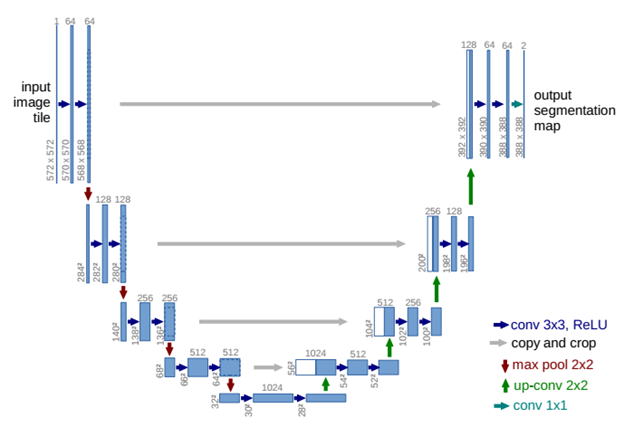
\includegraphics[width=14cm]{images/medicine/img3.png}
    \caption{Kiến trúc mô hình mạng Unet \cite{Unet}.}
\end{figure}

\begin{itemize}
    \item Phần mã hóa (Encoder):\\
    Bao gồm 3 phép ReLU, max pooling, convolution. Ở mỗi phép tích chập, Unet sử dụng kernel size (3x3) và unpadded convolution, tiếp theo sau tích chập là phép ReLU (rectified linear unit) và phép max pooling (2x2) với stride bằng 2 để giảm kích thước mẫu. Sau mỗi bước giảm kích thước mẫu, ta tiến hành nhân đôi số feature channels. 
    
    \item Phần giải mã (Decoder):\\
    Mỗi bước trong phần giải mã bao gồm một phép upsampling  của feature map, tiếp theo là một phép tích chập với kernel size (2x2), sau đó giảm số feature channels xuống một nửa. Mỗi phép concatenation sẽ kết hợp feature map ở phần giải mã với feature map tương ứng ở phần mã hóa (đã được copy và crop). Sau đó thực hiệp phép ReLU. 
\end{itemize}

\newpage

\subsection{Quá trình huấn luyện và hàm lỗi}
Hàm năng lượng $E$ được tính bởi pixel-wise soft-max trên feature map cuối cùng dựa trên hàm đánh giá mất mát cross entropy có trọng số. Hàm  cross entropy có trọng số sẽ phạt từng pixel dự đoán theo công thức.
\begin{equation}
    E = -\sum_{x \epsilon \Omega}^{ } w(x)\mathrm{log}(p(x))
\end{equation}
\begin{itemize}
\setlength\itemsep{5mm}
    \item $p(x)$ là giá trị xác xuất dự đoán cho đối tượng của pixel tại vị trí x.
    \item $\omega(x)$ là giá trị trọng số mà Olaf và các cộng sự đã giới thiệu để tăng cường độ quan trọng của từng pixel. 
\end{itemize}

Bởi vì mục tiêu của mô hình Unet là phân đoạn tế bào nên thách thức lớn nhất của chúng là tìm được biên phân chia giữa các tế bào một cách hiệu quả nhất. Do đó tác giả sẽ tăng cường mức phạt nếu vị trí pixel đó là biên phân chia giữa 2 đối tượng tế bào bằng kỹ thuật touching cells. 

Biểu đồ trọng số  được tính như sau:
\begin{equation}
    \omega(x) = \omega_{c}(x) + \omega_{0}.\mathrm{exp}\left(-\frac{(d_{1}(x) + d_{2}(x) )^{2}}{2\sigma^{2}} \right)
\end{equation}
\begin{itemize}
    \item $\omega_{c}: \Omega \rightarrow \mathbb{R}$ là trọng số để cân bằng dựa trên tỉ lệ của nhãn và nền. 
    \item $d_{1}: \Omega \rightarrow \mathbb{R}$ là khoảng cách từ pixel đến đối tượng tế bào (cell) gần nhất.
    \item $d_{2}:  \Omega \rightarrow \mathbb{R}$ là khoảng cách từ pixel đến đối tượng tế bào (cell) gần thứ 2.
    \item $\omega_0$: là trọng số quan trọng của khoảng cách pixel đến biên đóng góp cho hàm loss ($\omega_0 = 10$).
\end{itemize}

\begin{figure}[H]
    \centering
    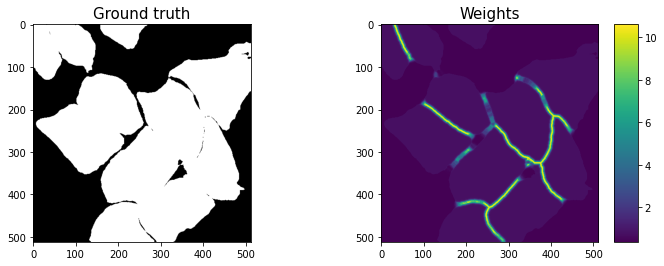
\includegraphics[width=14cm]{images/experience/w_unet.png}
    \caption{Hình minh họa cho ma trận trọng số được sinh ra từ nhãn}
\end{figure}
Tuy nhiên, bởi vì đây là bài toán tìm ranh giới giữa các tế bào nên việc nâng trọng số các pixel phân cách giữa các tế bào trở nên hiệu quả. Còn đối với bài toán phân đoạn gan và mạch máu thì việc sử dụng hàm đánh giá có trọng số như trên chưa được hiệu quả bởi đối với bài toán gan thì ảnh nó chỉ chứa 1 đối tượng gan ở 1 lát cắt nên việc đó sẽ không tìm ra ma trận trọng số ranh giới cho nó, còn đối với mạch máu thì không có nhiều ranh giới giữa các mạch máu với nhau mà nếu có thì cũng ít bị sát cạnh nhau như bài toán phân đoạn tế bào. Do đó chưa thể sử dụng hàm đánh giá có trọng số này trong bài toán phân đoạn gan và mạch máu.

\section{Mô hình Unet3D}
\label{sec:Unet3D}
Dựa trên sự thành công của mô hình Unet2D do Olaf \cite{Unet} đề xuất, kiến trúc Unet3D được sinh ra bởi \cite{unet3d} cũng đã đem lại nhiều kết quả khả quan đối với dữ liệu 3 chiều. Mô hình Unet3D dựa trên ý tưởng trước đó về kiến trúc chữ U gồm 2 nhánh: nhánh mã hóa mà nhánh giải mã. Tuy nhiên khác với phiên bản 2D , phiên bản này sẽ sử dụng các tác vụ 3D: Convolution 3D, Maxpooling 3D, và Transposed Convolution 3D. Unet3D sẽ nhận vào giá trị đầu vào có là các khối 3D và kết quả phân đoạn đầu ra là các khối 3D có cùng kích thước ứng với các nhãn cho từng pixel của khối 3D đó.

Kiến trúc mạng Unet3D được minh họa như hình \ref{unet3d_arch}. Trong mỗi khối tính toán được ký hiệu x@y với x là số lượng đặc trưng mà khối này trích xuất, y là kích thước bộ lọc tích chập.

\begin{figure}[H]
    \centering
    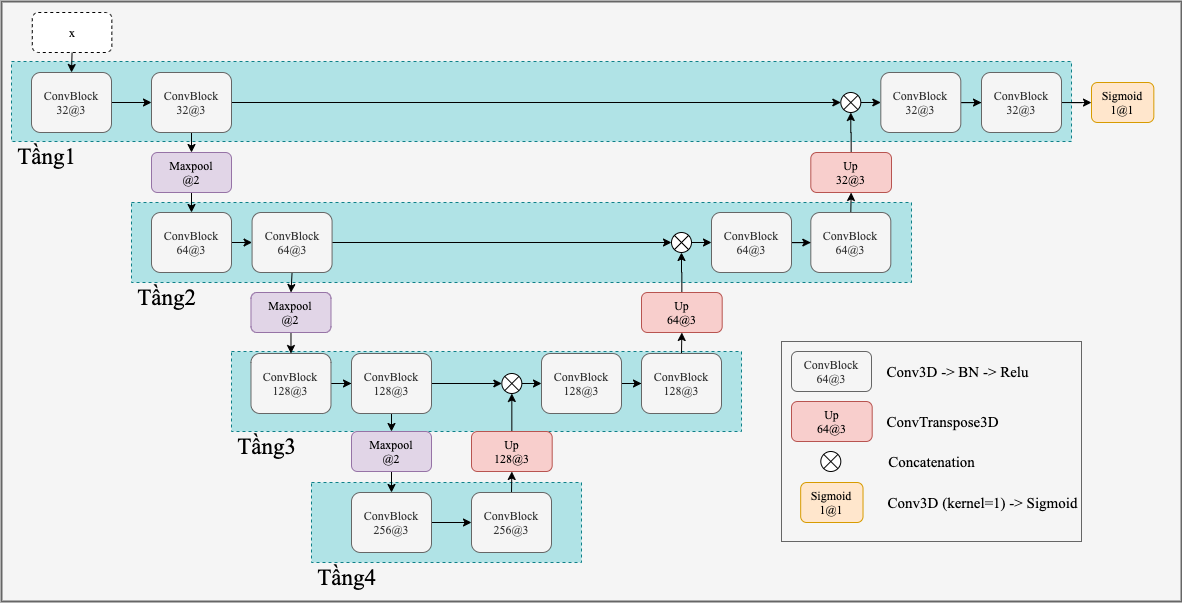
\includegraphics[width=14cm]{images/blood/model-Unet3D.png}
    \caption{Mô hình Unet3D 4 tầng}
    \label{unet3d_arch}
\end{figure}

Về mặt tổng quan kiến trúc này không khác nhiều so với kiến trúc mô hình Unet2D, tuy nhiên để ứng dụng vào các bài toán cụ thể khác nhau, chúng ta cần sử dụng các siêu tham số như số tầng phù hợp bởi kích thước các đối tượng của bài toán. Đối với những đối tượng bài toán rất nhỏ như mạch máu, việc mô hình càng sâu đặc trưng thu được sẽ càng có tính toàn cục điều này khiến cho các vùng chứa mạch máu có thể bị phá vỡ.\par


\section{Mô hình TLUnet3D} \label{bg-TLUnet3D}
Mô hình TLUnet3D được giới thiệu trong \cite{LV_LIVER} là một biến thể của mô hình Unet3D sử dụng phương pháp học chuyển tiếp (transfer learning) để cải thiện kết quả phân đoạn. Đây là phương pháp sử dụng lại trọng số của một số lớp, hoặc toàn bộ các lớp của một mô hình đã được huấn luyện trước đó để khởi tạo cho các lớp trên mô hình mới.\par
Mô hình TLUnet3D gồm ba phần: mã hóa, giải mã và nối tắt. Phần mã hóa sử dụng lại kiến trúc và trọng số của mô hình tích chập 3 chiều (CNN3D) hay nói cách khác, mô hình CNN3D cần được huấn luyện trước mô hình TLUnet3D. Kiến trúc mô hình CNN3D như sau:
\begin{figure}[H]
    \centering
    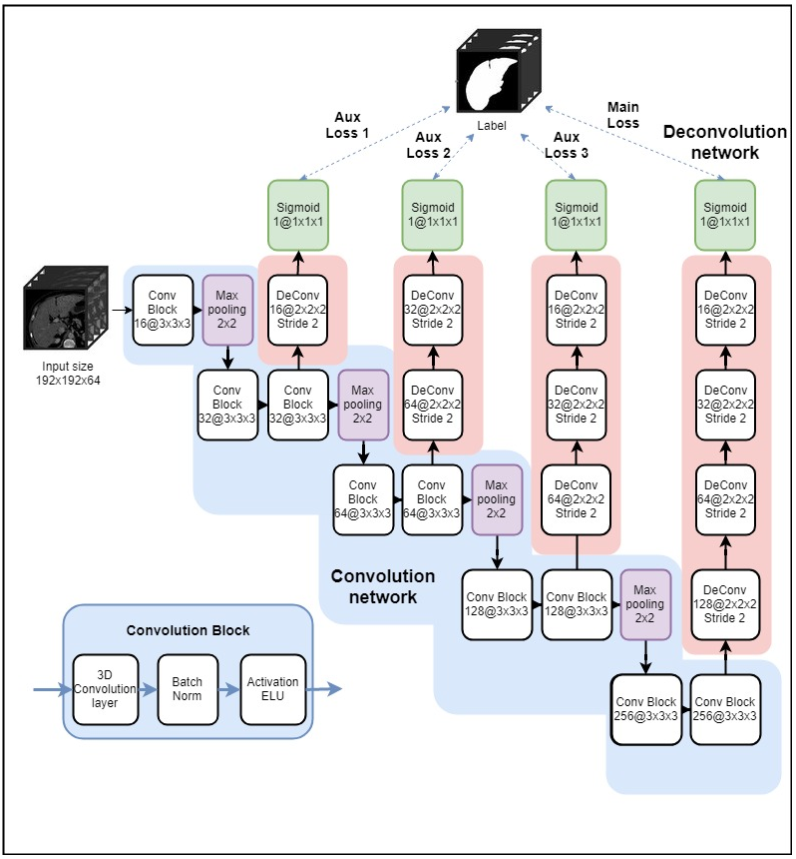
\includegraphics[width=12cm]{images/liver/CNN3D/CNN3D.png}
    \caption{Kiến trúc mô hình CNN3D\cite{LV_LIVER}}
    \label{fig:CNN3D}
\end{figure}
Hàm mất mát của mô hình CNN3D được tính từ hàm mất mát của tất cả các phần giải mã:
\begin{align}
    \label{LossCNN3D}
    Loss = \mu_{1}Loss_{aux1} + \mu_{2}Loss_{aux2} + \mu_{3}Loss_{aux3} + \mu_{4}Loss_{main}
\end{align}
\textbf{Cơ chế giám sát sâu (Deep supervision)} được đề xuất năm 2016 \cite{Deepsupervision} bởi Qi Dou và cộng sự đã được tác giả kế thừa trong quá trình huấn luyện mô hình CNN3D. Cơ chế giám sát sâu giúp mô hình học tập hiệu quả và đem lại kết quả tốt hơn so với phương pháp học thông thường. Thông qua việc sử dụng thêm các cổng ra tại từng tầng của giai đoạn mã hóa, trọng số của các lớp tính toán sẽ được cập nhập và chia sẻ thông tin với nhau giữa các luồn thay vì chỉ chạy xuyên qua 1 luồn chính như mô hình gốc Unet. Nhờ vào đó, đặc trưng trích xuất qua từng tầng của giai đoạn mã hóa sẽ trở nên trừu tượng có ích hơn vì chúng được kiểm tra song song với giá trị cuối cùng. Về hàm lỗi, tác giả đã sử dụng hàm Binary Cross-Entropy để huấn luyện mô hình với các siêu tham số $\mu_{1} = 1$,  $\mu_{2} = 2$,  $\mu_{3} = 4$,  $\mu_{4} = 8$. 

Khác biệt thứ 2 là ở phần nối tắt của mô hình TLUnet3D, tác giả đã thêm một lớp tích chập với kích thước cửa sổ 5x5 vào phần nối tắt để giảm số kênh (channel) trước khi kết hợp với kết quả lớp đảo tích chập tương ứng. Phần giải mã tương tự như phần giải mã của mô hình Unet3D nhưng được chỉnh sửa số lượng kênh.

Khi huấn luyện mô hình TLUnet3D, chỉ có phần giải mã và nối tắt được huấn luyện, trọng số của phần mã hóa được đóng băng. Mô hình được huấn luyện với số lượng dữ liệu ít hơn lúc huấn luyện mô hình CNN3D để tránh xảy ra hiện tượng quá khớp (overfitting). Kiến trúc mô hình cụ thể tại Hình \ref{tlunet}.

Ở bước tiền xử lý dữ liệu, tác giả sử dụng công cụ Anisotropic diffusion filter trong thư viện SimpleItk để loại bỏ nhiễu. Việc này mất khá nhiều thời gian nhưng đem lại kết quả tốt.

Kỹ thuật hậu xử lý tìm thành phần liên thông lớn nhất (gan) sau đó loại bỏ các thành phần còn lại (loại bỏ khối) cùng với kỹ thuật lấp đầy khối cũng được tác giả sử dụng. Việc áp dụng hậu xử lý giúp cải thiện kết quả phân đoạn gan.

\begin{figure}[H]
    \centering
    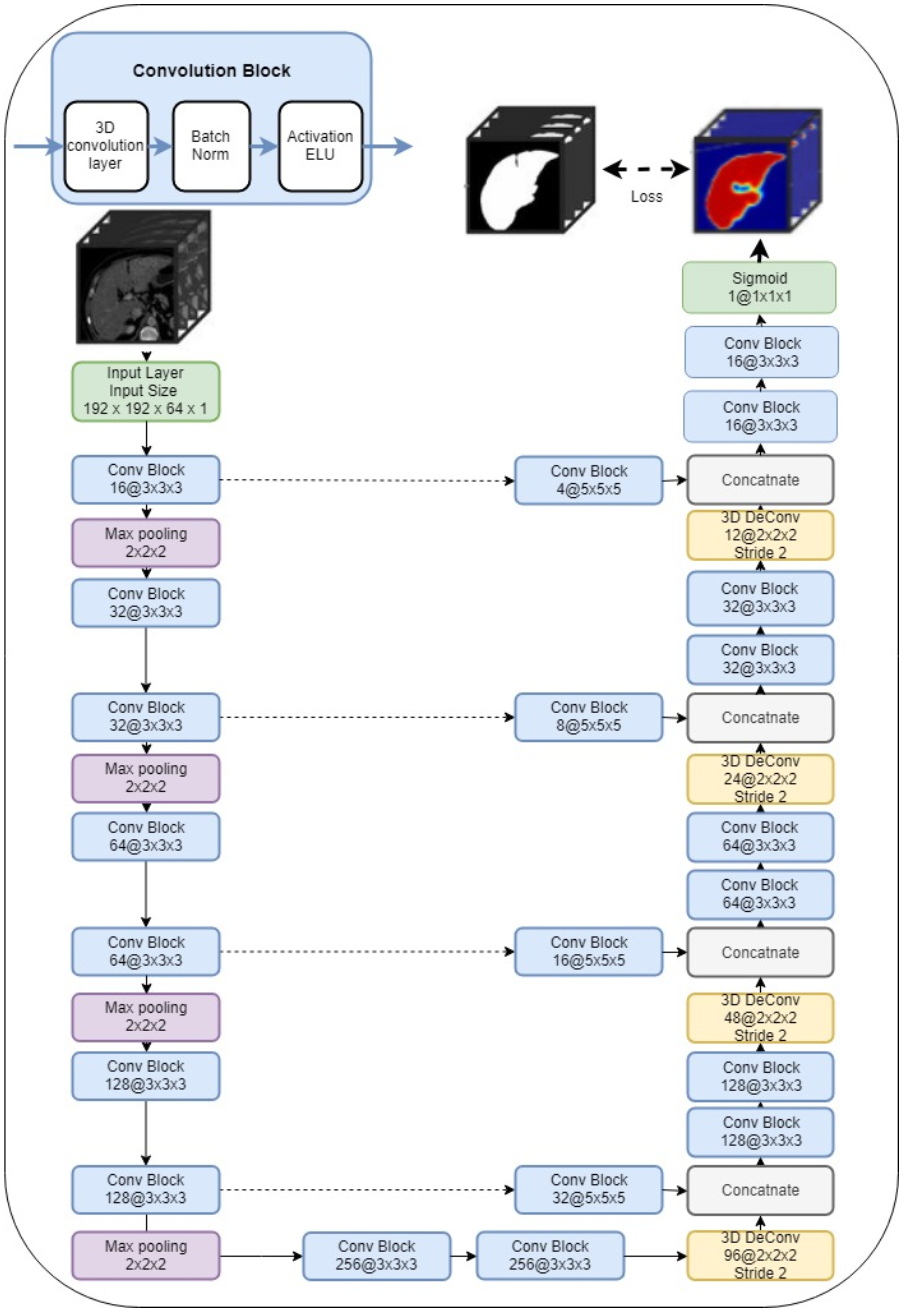
\includegraphics[width=14cm]{images/liver/TLUnet3D/TLUnet3D.png}
    \caption{Kiến trúc mô hình TLUnet3D\cite{LV_LIVER}}
    \label{tlunet}
\end{figure}

\begin{figure}[H]
    \centering
    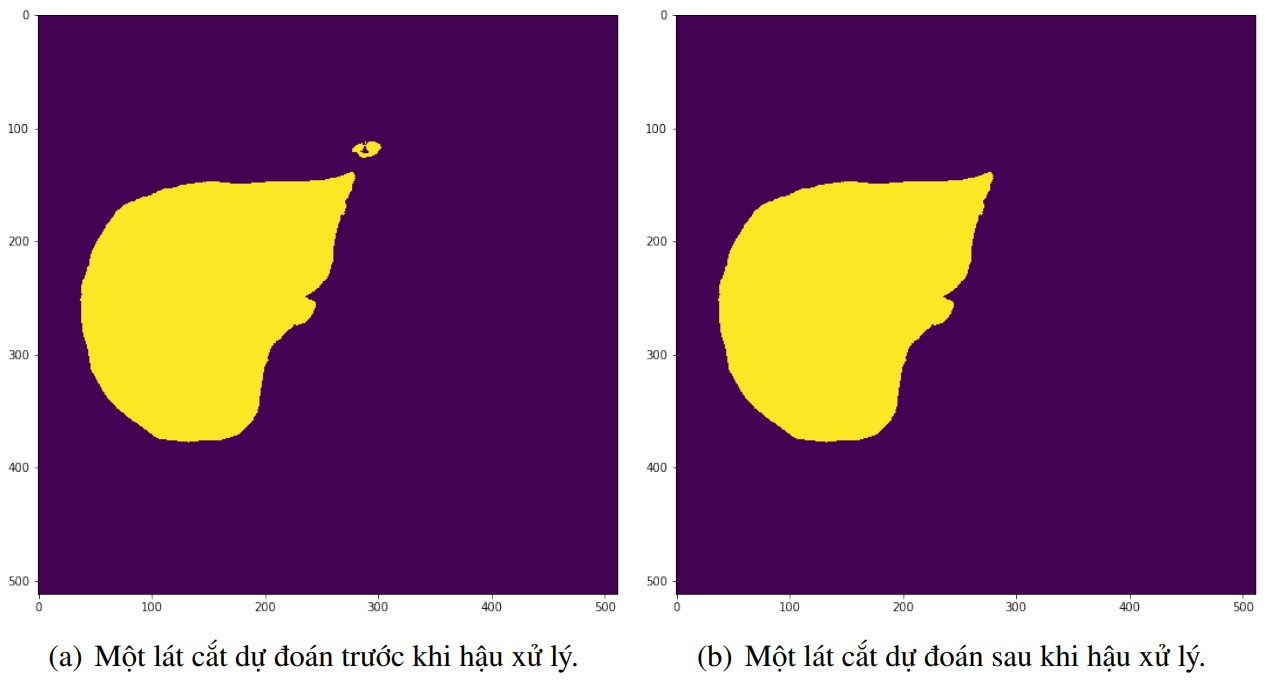
\includegraphics[width=12cm]{images/liver/TLUnet3D/posprocessing.jpg}
    \caption{Thay đổi của một dự đoán trước và sau hậu xử lý \cite{LV_LIVER}}
    \label{posprocessing}
\end{figure}
\vspace{-5mm}
Thực tế, mô hình CNN3D được huấn luyện trên ba tập dữ liệu Sliver07, Lits17 và 3Dircadb đã đem lại kết quả tốt, mô hình TLUnet3D giúp làm mượt (fine-tune) trên từng tập để cải thiện kết quả trên từng tập dữ liệu tương ứng. Mô hình TLUnet3D cho kết quả Dice cải thiện khoảng 1\% trên từng tập so với mô hình CNN3D theo công bố của tác giả. 

\newpage

\section{Mô hình U\textsuperscript{2}net}
Mô hình mạng U\textsuperscript{2}net được giới thiệu trong bài báo \cite{u2-net} bởi Qin và cộng sự vào năm 2020. Bài toán mà tác giả hướng đến là phát hiện đối tượng nổi bật nhất trong ảnh (Salient object detection - SOD). Tuy đây không phải là bài toán phân đoạn ảnh y khoa nhưng về phương pháp đều là gắn nhãn cho từng điểm ảnh thuộc đối tượng nổi bật (foreground) hoặc là nền (background). Điều này khá tương đồng với bài toán phân đoạn, và mô hình này đã đạt được kết quả cao nhất trong các mô hình hiện đại (state of the art) trong lĩnh vực SOD với chỉ số $F_{measure}$ đạt trên 95\% (Hình \ref{BenU2net}). Thứ hai, mô hình mà tác giả sử dụng là biến thể của mạng Unet (mô hình backbone được nhóm tập trung cải thiện), do đó đây là bài báo đáng được tham khảo.

\begin{figure}[H]
	\begin{center}
		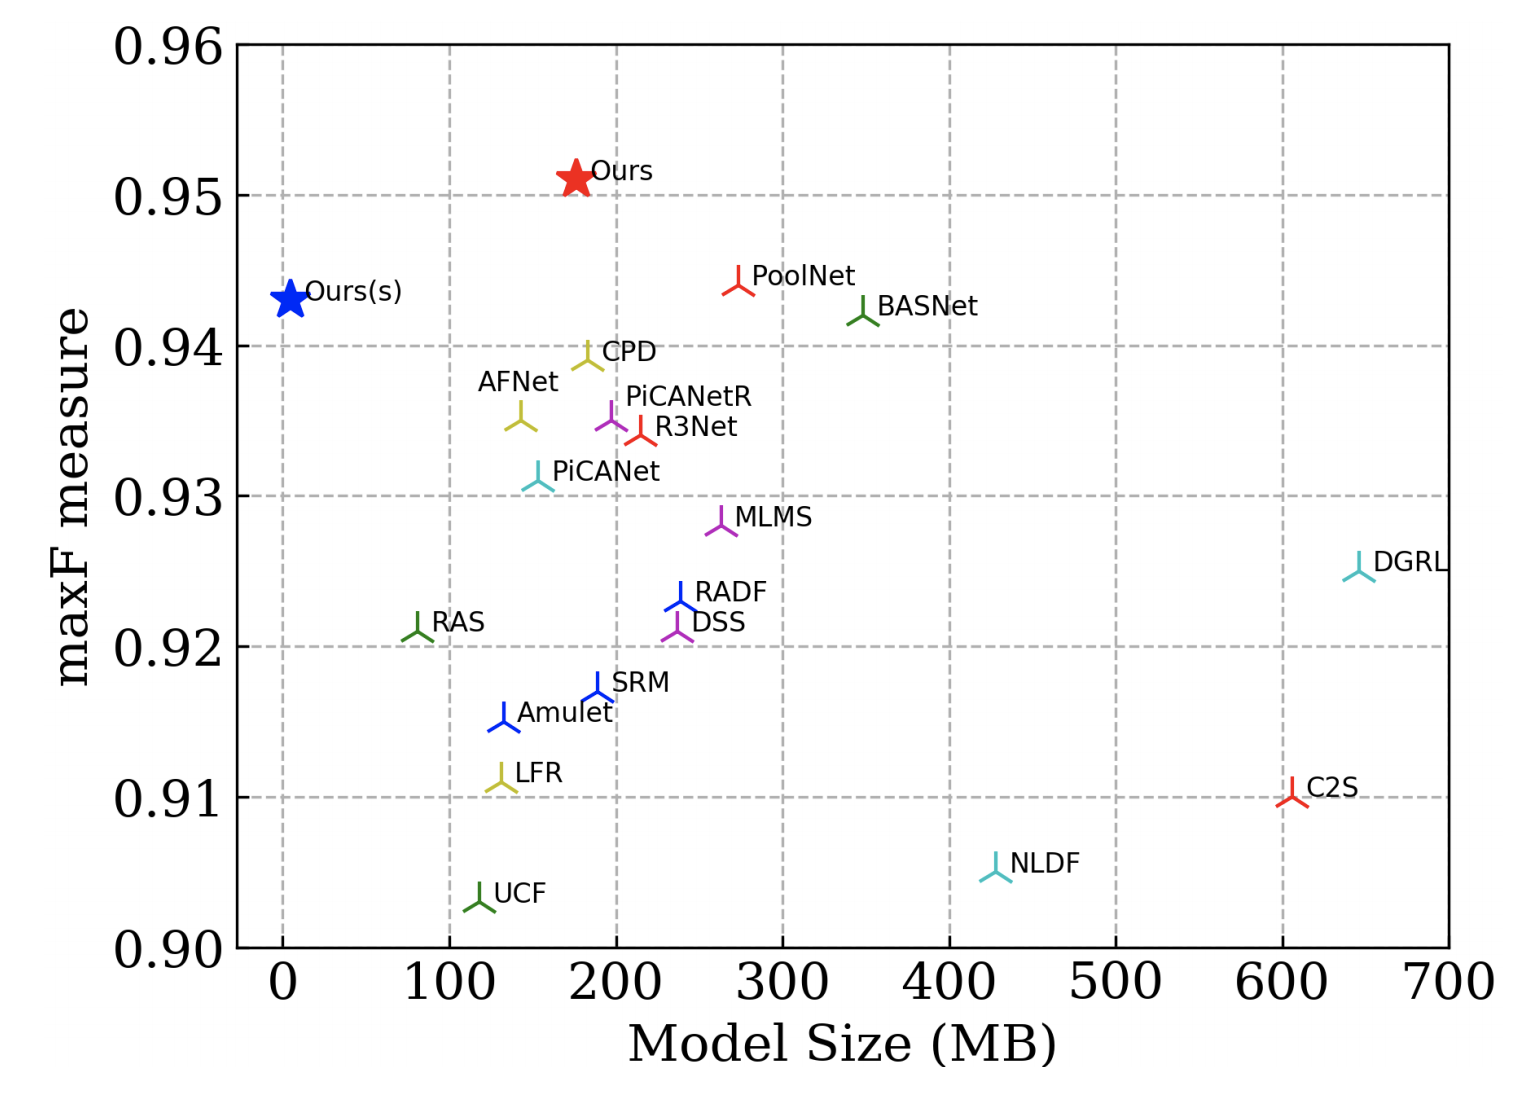
\includegraphics[width=8cm]{images/blood/u2_benk.png}
		\caption{So sánh mức độ hiệu quả U2net và các mô hình các trong lĩnh vực SOD\cite{u2-net}.}
		\label{BenU2net}
	\end{center}
\end{figure}
\vspace{-1.0cm}

\subsection{Hướng tiếp cận}
Bất lợi của các mô hình phân đoạn hiện nay, các đặc trưng mang thông tin toàn cục nhiều sẽ được mô hình trích xuất ở các lớp sâu hơn (thông thường sẽ qua các lớp gộp để giảm chi phí tính toán). Do đó khi chạy qua các lớp sâu thường sẽ khiến kích thước các đặc trưng giảm dần qua từng tầng và chúng mới mang lại nhiều thông tin ngữ cảnh toàn cục. Trong khi đó việc các đặc trưng mang tính ngữ cảnh toàn cục hay cục bộ đều rất quan trọng trong việc dự đoán điểm ảnh đó có thuộc đối tượng cần dự đoán hay không bởi các đối tượng có nhiều kích thước khác nhau. Với bất lợi đó nên các mô hình hiện tại chỉ đi sâu với một số tầng nhất định. Để giải quyết bất lợi đó, tác giả đã đề xuất một kiến trúc khối giúp cho việc có thể cho các đặc trưng đi sâu hơn qua các lớp mà vẫn giữ được kích thước đặc trưng ban đầu của chúng đó là khối Residual U-block.

\subsection{Khối Residual U-block - RSU}
Sự khác biệt đầu tiên giữa khối RSU với các khối tích chập thông thường là nhánh kết nối tắt, tác giả đã có sự cải tiến so với phép lấy phần dư được giới thiệu trong mạng phần dư (ResNet) \cite{resnet} được giới thiệu năm 2015. Thay vì sử dụng lại giá trị đầu vào ban đầu, tác giả đã sử dụng một tầng tích chập để trích xuất các đặc trưng cục bộ, rồi truyền nó thông qua phép nối tắt xuyên qua một hay nhiều lớp như hình \ref{RSB}.b.

\begin{figure}[H]
	\begin{center}
		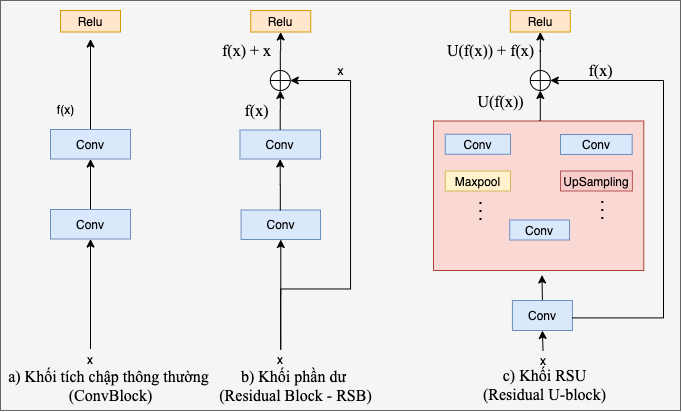
\includegraphics[width=10cm]{images/blood/compareRSU.png}
		\caption{So sánh giữa khối Residual U-Block(RSU) và  các khối tích chập phổ biến. }
		\label{RSB}
	\end{center}
\end{figure}
\vspace{-1.0cm}
Thứ hai, lấy ý tưởng từ mô hình Unet \cite{Unet}, một kiến trúc chữ gồm 2 phần: phần mã hóa và phần giải mã, đặc trưng đầu vào sẽ được mã hóa thông qua nhiều tầng khác nhau sau đó được giải mã về kích thước ban đầu. Nhờ vào đó đặc trưng được trích xuất từ khối tính toán này sẽ mang nhiều thông tin ngữ cảnh toàn cục hơn so với khối tích chập thông thường, bởi việc nó trích xuất thông tin dựa trên những kích thước khác nhau qua từng tầng trích xuất. Sau đó được giải mã về kích thước ban đầu, điều này giúp cho các đặc trưng sau khi qua khối RSU sẽ còn có kích thước đủ lớn để đi sâu thêm những tầng về sau.

Tổng hợp 2 ý tưởng, khối RSU sẽ đem lại vừa là thông tin toàn cục (bởi việc đi sâu xuống tầng mã hóa) vừa là thông tin cục bộ (nhờ vào tầng tích chập đầu tiên) được kết hợp lạị với nhau. Kiến trúc khối U-Block được trình bày như hình \ref{rsu}.

\begin{figure}[H]
	\begin{center}
		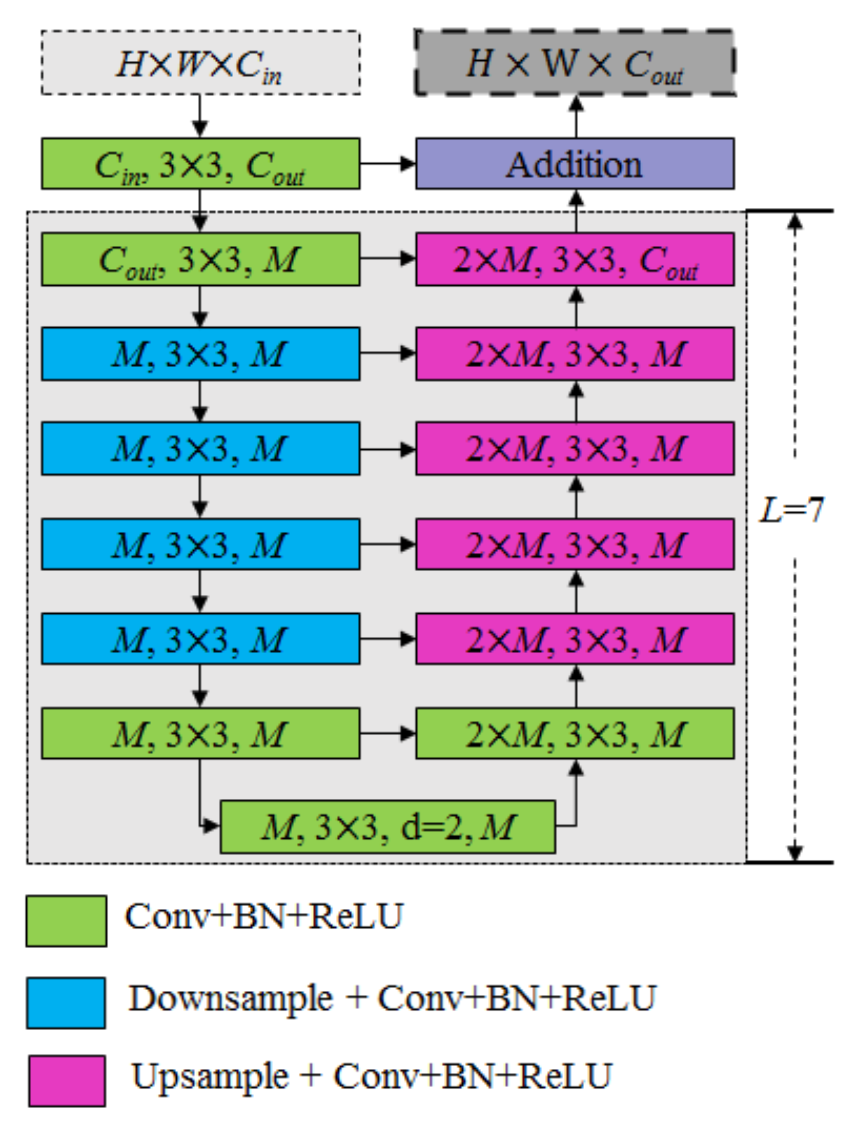
\includegraphics[width=8cm]{images/blood/RSU.png}
		\caption{Kiến trúc khối Residual U-block (RSU)\cite{u2-net}. }
		\label{rsu}
	\end{center}
\end{figure}
\vspace{-1.0cm}

Một khối RSU sẽ có 3 siêu tham số: $\mathrm{C_{in}, C_{out}, L}$ tương ứng với số kênh đầu vào/đầu ra và độ sâu của mạng. Một khối có kiến trúc đối xứng giữa phần mã hóa và phần giải mã với độ sâu L với mục tiêu trích xuất thông tin ngữ cảnh thông qua từng kích thước đặc trưng khác nhau (multi-scale contextual information) được ký hiệu U(F(x)). Với F(x) là đặc trưng cục bộ được trích xuất đầu tiên nhờ vào tầng tích chập. Độ sâu L càng lớn, càng nhiều phép gộp được sử dụng nhờ đó tăng vùng nơron nhìn thấy (receptive field) giúp làm giàu thông tin ngữ cảnh toàn cục hơn. Ký hiệu M là siêu tham số của khối RSU, đại diện số lượng các đặc trưng được trích xuất qua mỗi tầng tích chập.

\subsection{Kiến trúc mạng}
Kiến trúc mạng U\textsuperscript{2}net sẽ có kiến trúc tổng quan giống như mạng Unet bao gồm 2 nhánh: nhánh mã hóa và nhánh giải mã.

\begin{figure}[H]
	\begin{center}
		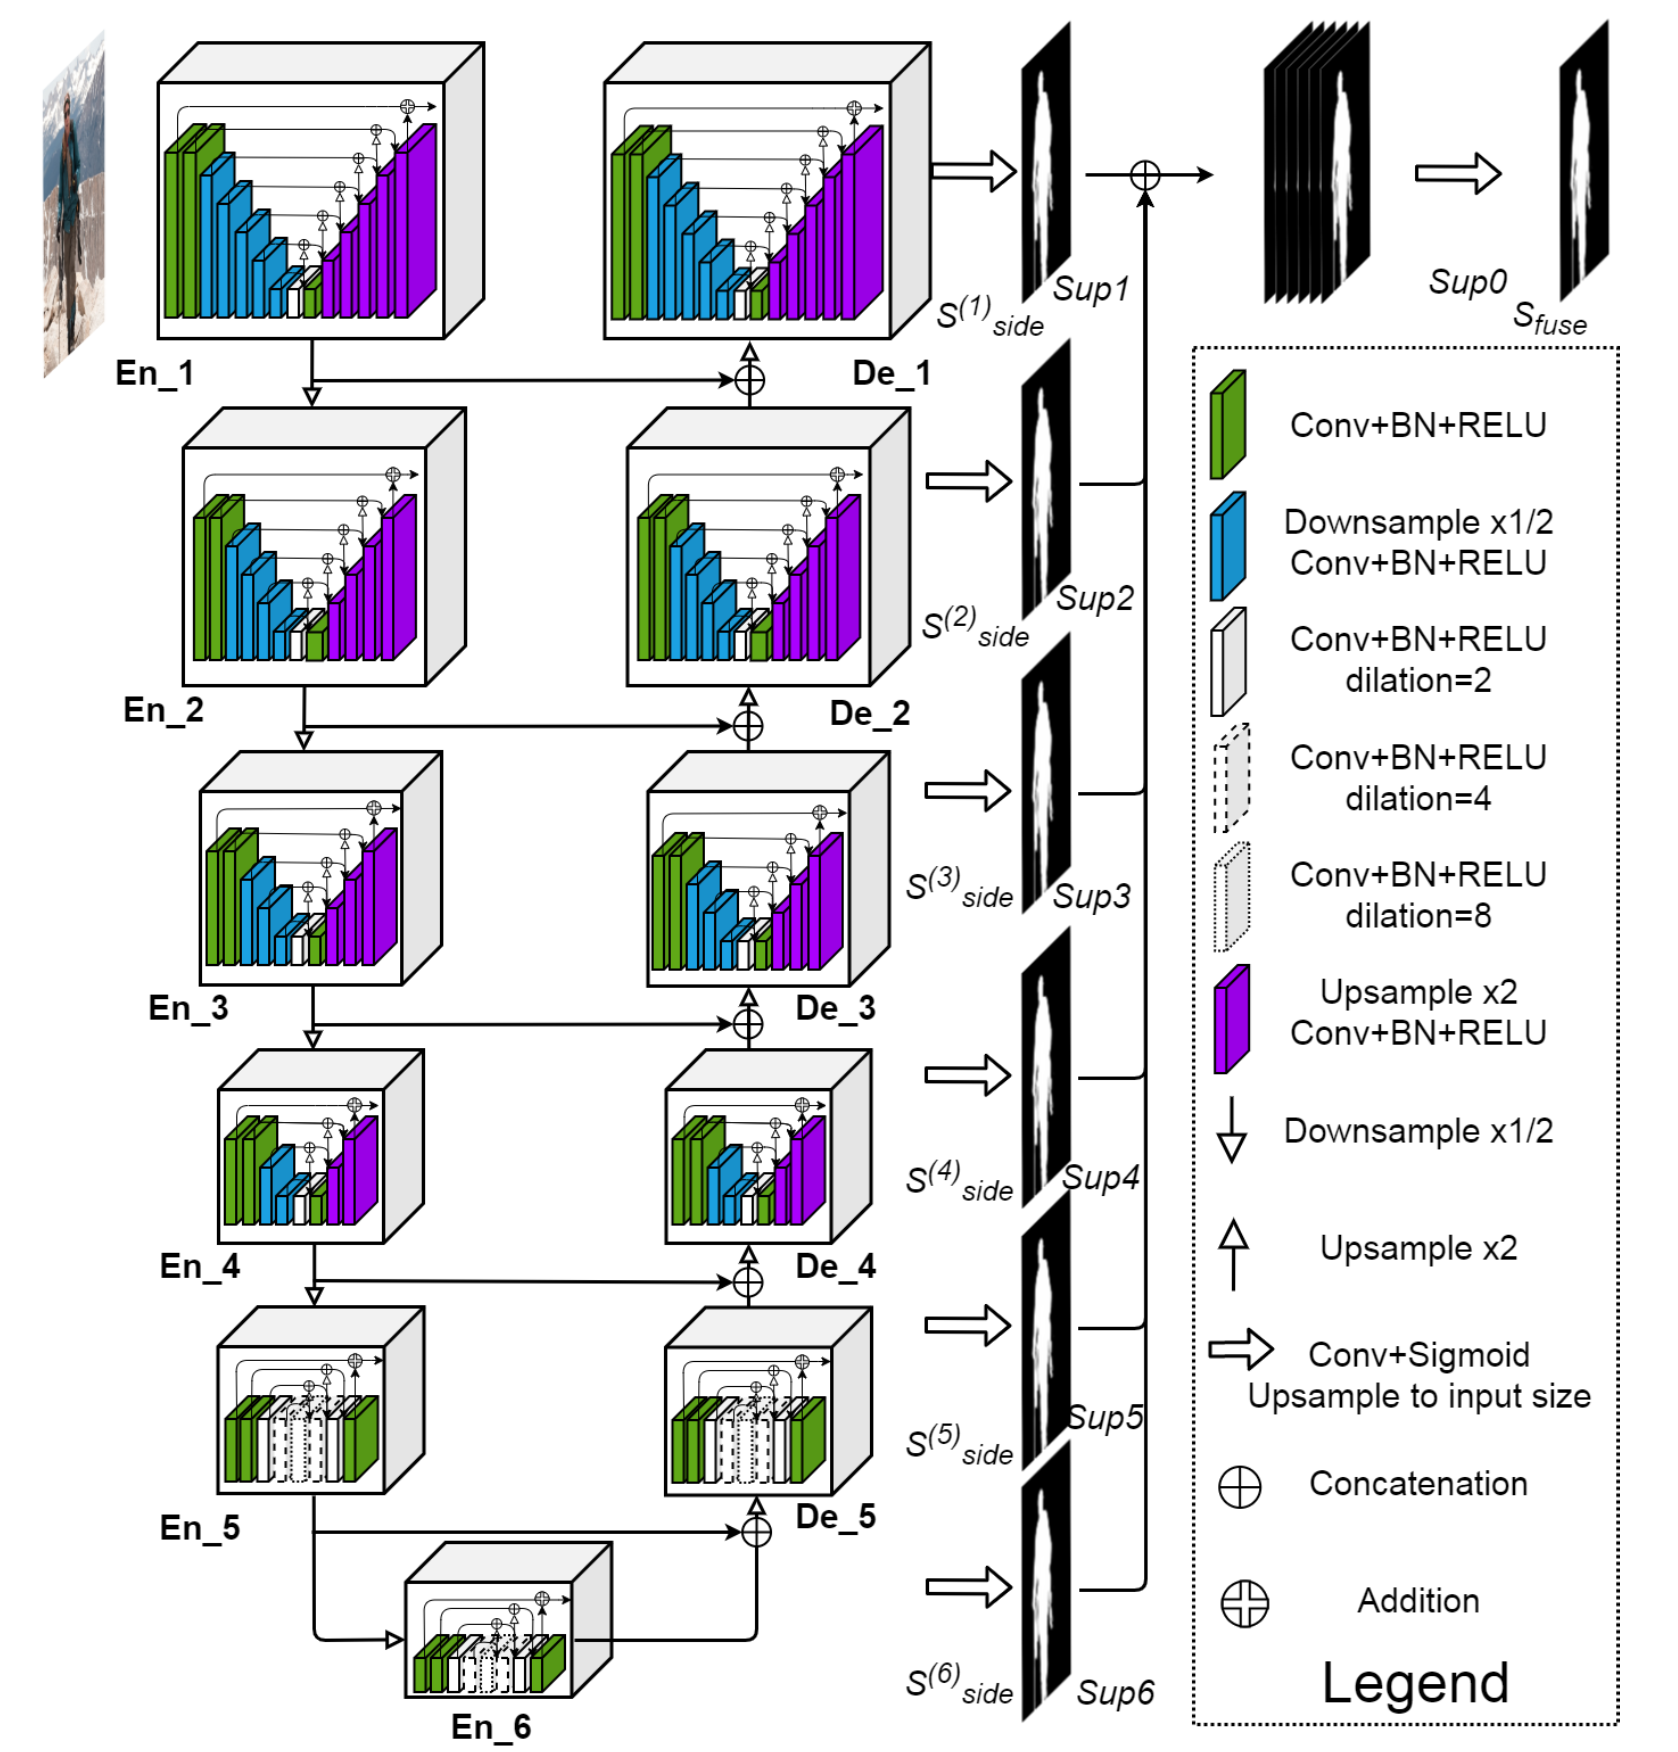
\includegraphics[width=12cm]{images/blood/u2net_paper.png}
		\caption{Kiến trúc mô hình U\textsuperscript{2}net\cite{u2-net}. }
		\label{u2net_arch}
	\end{center}
\end{figure}
\vspace{-1.0cm}

Thay bằng việc sử dụng các khối tích chập thông thường tác giả đã sử dụng khối Residual U-block được giới thiệu ở trên để tạo thành bộ mã hóa và giải mã tương ứng. Mô hình có độ sâu là 6: gồm 6 tầng tương ứng với 5 phép gộp đối xứng với 5 phép upsample (không có trọng số). Qua mỗi tầng kích thước các đặc trưng thu được sẽ giảm đi một nữa. Tại mỗi tầng sẽ bao gồm 2 khối RSU (1 khối tại phần mã hóa, 1 khối tại phần giải mã). Mỗi khối RSU sẽ có độ sâu là L. Tương ứng với mỗi tầng độ sâu khối L sẽ có giá trị giảm dần 1 đơn vị, tại tầng đầu tiên (En\_1) khối RSU sẽ có L=7, tại tầng thứ 2 sẽ có L=6 cho đến tầng cuối cùng. Mô hình có sử dụng phép kết nối tắt (skip connection) giữa bộ mã hóa (encoder) và bộ giải mã (decoder) với mục tiêu trong quá trình khôi phục kích thước tại mỗi tầng, đặc trưng sẽ được kết hợp với thông tin mã hóa ban đầu nhằm tăng tính ngữ cảnh . Bên cạnh đó việc sử dụng các phép kết nối tắt giúp cho mô hình tránh tình trạng đạo hàm bị tiêu biến (Vanishing Gradient).
